\documentclass[tikz]{standalone}
%\usepackage{fontawesome}

% \newfontfamily{\FA}{Font Awesome 5 Free} % some glyphs missing
\expandafter\def\csname faicon@facebook\endcsname{{\FA\symbol{"F09A}}}
\def\faQuestionSign{{\FA\symbol{"F059}}}
\def\faQuestion{{\FA\symbol{"F128}}}
\def\faExclamation{{\FA\symbol{"F12A}}}
\def\faUploadAlt{{\FA\symbol{"F093}}}
\def\faLemon{{\FA\symbol{"F094}}}
\def\faPhone{{\FA\symbol{"F095}}}
\def\faCheckEmpty{{\FA\symbol{"F096}}}
\def\faBookmarkEmpty{{\FA\symbol{"F097}}}

%\def\faCatt{{\FA\symbol{"F6BE}}}
%\def\faCat{\faicon{cat}}
%\def\faCat{\faicon{yoast}}
\expandafter\def\csname faicon@dog\endcsname{{\FA\symbol{"F4DA}}}
%\def\faDog{\faicon{dog}}
%\def\faDog{{\FA\symbol{"F4DA}}}
%\def\faDogg{{\FA\symbol{"F6D3}}}
%\def\faDogg{{\FA\symbol{"F596}}}

% /usr/share/texlive/texmf-dist/fonts/opentype/public/fontawesome5/FontAwesome5Free-Solid-900.otf
\newfontfamily{\FAS}{FontAwesome5Free-Solid-900.otf}
%\expandafter\def\csname faicon@download\endcsname{{\FAS\symbol{"F6D3}}}
\expandafter\def\csname faicon@cat\endcsname{{\FAS\symbol{"F6BE}}}
\def\faCat{\faicon{cat}}
\expandafter\def\csname faicon@dog\endcsname{{\FAS\symbol{"F6D3}}}
\def\faDog{\faicon{dog}}
\expandafter\def\csname faicon@dragon\endcsname{{\FAS\symbol{"F6D5}}}
\def\faDragon{\faicon{dragon}}
\expandafter\def\csname faicon@fish\endcsname{{\FAS\symbol{"F578}}}
\def\faFish{\faicon{fish}}
\expandafter\def\csname faicon@horse\endcsname{{\FAS\symbol{"F6F0}}}
\def\faHorse{\faicon{horse}}
\expandafter\def\csname faicon@spider\endcsname{{\FAS\symbol{"F717}}}
\def\faSpider{\faicon{spider}}

\expandafter\def\csname faicon@chessking\endcsname{{\FAS\symbol{"F43F}}}
\def\faChessKing{\faicon{chessking}}
\expandafter\def\csname faicon@chessqueen\endcsname{{\FAS\symbol{"F445}}}
\def\faChessQueen{\faicon{chessqueen}}
\expandafter\def\csname faicon@chessrook\endcsname{{\FAS\symbol{"F447}}}
\def\faChessRook{\faicon{chessrook}}
\expandafter\def\csname faicon@chesspawn\endcsname{{\FAS\symbol{"F443}}}
\def\faChessPawn{\faicon{chesspawn}}
\expandafter\def\csname faicon@chessknight\endcsname{{\FAS\symbol{"F441}}}
\def\faChessKnight{\faicon{chessknight}}
\expandafter\def\csname faicon@chessbishop\endcsname{{\FAS\symbol{"F43A}}}
\def\faChessBishop{\faicon{chessbishop}}
\expandafter\def\csname faicon@chess\endcsname{{\FAS\symbol{"F439}}}
\def\faChess{\faicon{chess}}







\usepackage{tikz}
\usetikzlibrary{positioning,trees,decorations.pathreplacing}

\begin{document}
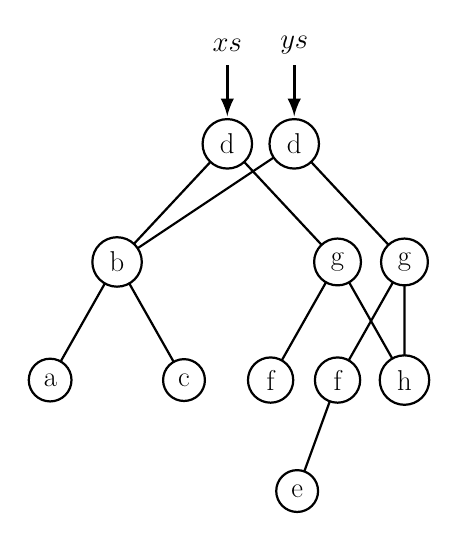
\begin{tikzpicture}[thick,scale=0.5, every node/.style={scale=0.5},level distance=3cm]
    \tikzstyle{marrs}=[very thick,-latex]
    \tikzstyle{tnode}=[circle, draw=black,node distance=1.7cm]
    \tikzstyle{level 1}=[sibling distance=5.6cm]
    \tikzstyle{level 2}=[sibling distance=3.4cm]
    
    \huge

    \draw (0, 2.5) node {$xs$};
    \draw[marrs] (0, 2) -- +(0, -1.3);
    
    \draw (1.7, 2.5) node {$ys$};
    \draw[marrs] (1.7, 2) -- +(0, -1.3);
    
    \node[tnode] (n_d) {d}
    child {node[tnode] (n_b) {b}
        child {node[tnode] (n_a) {a}}
        child {node[tnode] (n_c) {c}}
    }
    child {node[tnode] (n_g) {g}
        child {node[tnode] (n_f) {f}
        node[tnode] (n_f') [right of=n_f] {f} [clockwise from=250]
        child {node[tnode] (n_e) {e}}
        }
        child {node[tnode] (n_h) {h}}
        node[tnode] (n_g') [right of=n_g] {g}
    }
    node[tnode] (n_d') [right of=n_d]{d};
    
    \path (n_d') edge (n_b);
    \path (n_d') edge (n_g');
    \path (n_g') edge (n_f');
    \path (n_g') edge (n_h);
    
\end{tikzpicture}
\end{document}